% CS 221M Final Project Report — blogpost-style, 2 pages
% Build: latexmk -pdf main.tex   (or: make)
\documentclass[10pt]{article}

\usepackage[margin=0.7in,top=0.62in,bottom=0.62in]{geometry}
\usepackage[T1]{fontenc}
\usepackage{amsmath,amssymb}
\usepackage{graphicx}
\usepackage{parskip}
\usepackage{titlesec}
\usepackage[dvipsnames]{xcolor}
\usepackage[colorlinks=true,linkcolor=black,citecolor=gray,urlcolor=RoyalBlue]{hyperref}
\usepackage{caption}

\captionsetup{font=footnotesize,labelfont=bf,skip=3pt}
\titleformat{\section}{\large\bfseries}{}{0pt}{}
\titlespacing*{\section}{0pt}{8pt}{2pt}
\setlength{\parskip}{3pt}
\setlength{\textfloatsep}{8pt}
\setlength{\intextsep}{8pt}
\renewcommand{\topfraction}{0.92}
\renewcommand{\bottomfraction}{0.6}
\renewcommand{\textfraction}{0.05}
\renewcommand{\floatpagefraction}{0.85}

\newcommand{\repourl}{https://github.com/kirillacharya/manifold-steering-replication}

\begin{document}

\begin{center}
  {\LARGE\bfseries Replicating Manifold Steering:\\[2pt]
   Geometry of LLM Representations and Behavior}\\[5pt]
  {\normalsize Kirill Acharya \,·\, Stanford University \,·\, CS 221M Final Project}\\[2pt]
  {\small Code, checkpoints, and figures: \;\url{\repourl}}
\end{center}

\section{Background: do LLM representations and behavior share a geometry?}

Large language models build up internal representations layer by layer: at
layer $L$, each token maps to a hidden state $h^{(L)}\in\mathbb{R}^d$, and
structured concept domains may organize into geometric patterns. Hidden
states for \emph{days of the week} or \emph{months of the year} may trace a
smooth, low-dimensional manifold $\mathcal{M}_h\subset\mathbb{R}^d$ ---
closed loops for cyclic domains, open curves for sequential ones. Wurgaft et
al. [1] ask whether this geometry \emph{predicts
behavior}: output probability vectors, embedded via the Hellinger map
$p\mapsto\sqrt{p}$ (which makes the Hellinger distance
$d_H(p,q)=\tfrac{1}{\sqrt 2}\lVert\sqrt p-\sqrt q\rVert$ Euclidean
[2]), may trace a matching \emph{behavior manifold}
$\mathcal{M}_y$. If $\mathcal{M}_h\approx\mathcal{M}_y$ isometrically,
steering \emph{along} $\mathcal{M}_h$ should produce natural behavioral
transitions, while linear steering cuts off-manifold and ``teleports''
probability mass. The two strategies interpolate between a source concept
$\hat h_{c_s}$ and a target $\hat h_{c_e}$:
\[
  \pi_{\mathrm{lin}}(\alpha) = (1-\alpha)\,\hat h_{c_s} + \alpha\,\hat h_{c_e},
  \qquad
  \pi_{\mathrm{mfd}}(\alpha) = s\!\big((1-\alpha)\,u_{c_s} + \alpha\,u_{c_e}\big),
  \quad u_{c_i} = s^{-1}(\hat h_{c_i}),
\]
where $s:\mathbb{R}^k\to\mathbb{R}^d$ maps intrinsic coordinates back to
activation space. We replicate the paper's central figure on a small open
model, then extend it to a 2D concept structure (a day$\times$hour torus).

\begin{figure}[b!]
  \centering
  \begin{tabular}{@{}cc@{}}
    \multicolumn{2}{c}{\footnotesize\bfseries Weekdays \hspace{0.255\textwidth} Months}\\[-1pt]
    
\includegraphics[width=0.255\textwidth,trim=0 40pt 0 55pt,clip]{figures/weekdays_behavior.png} &
    
\includegraphics[width=0.255\textwidth,trim=0 40pt 0 55pt,clip]{figures/months_behavior.png}\\
    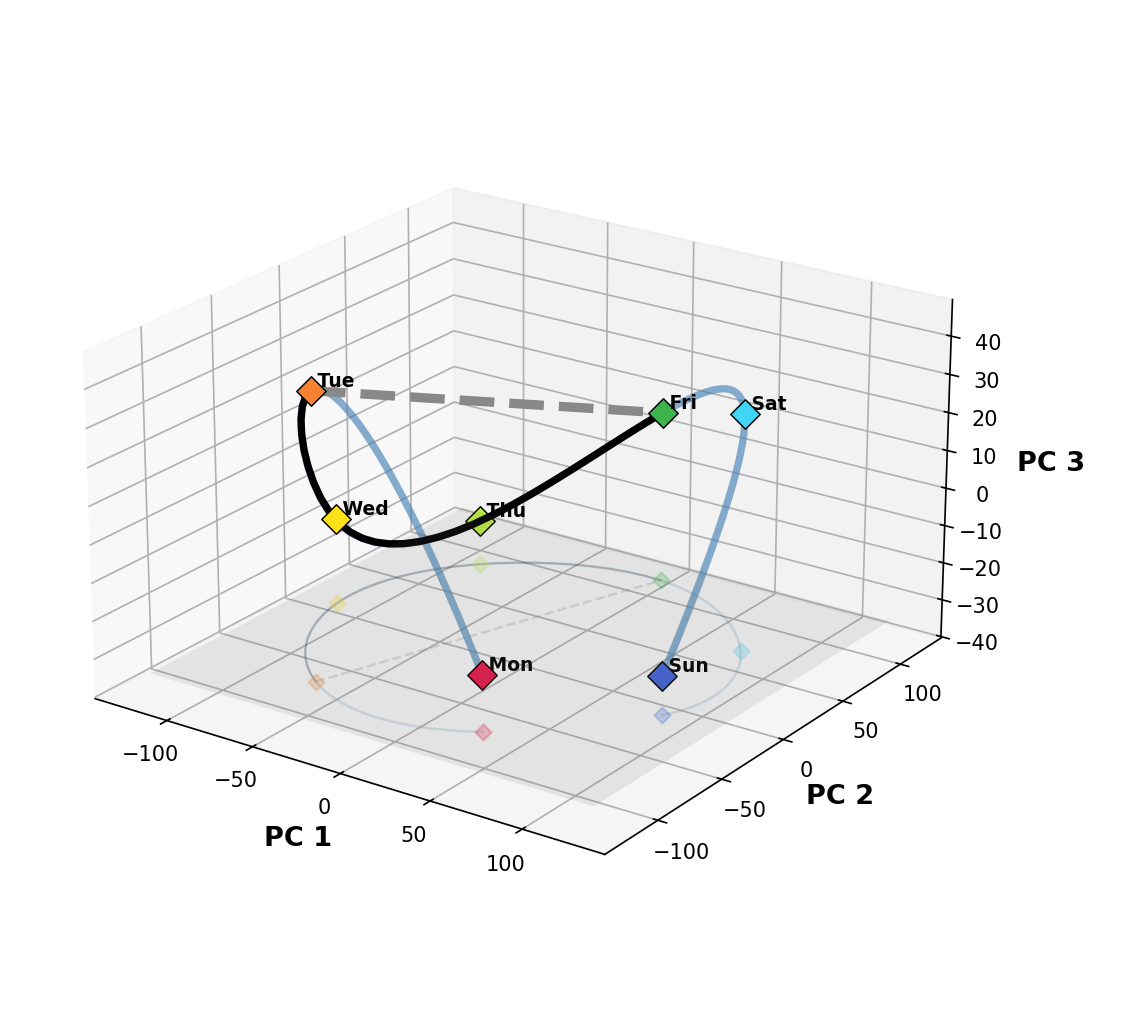
\includegraphics[width=0.255\textwidth,trim=0 0 0 55pt,clip]{figures/weekdays_activation.png} &
    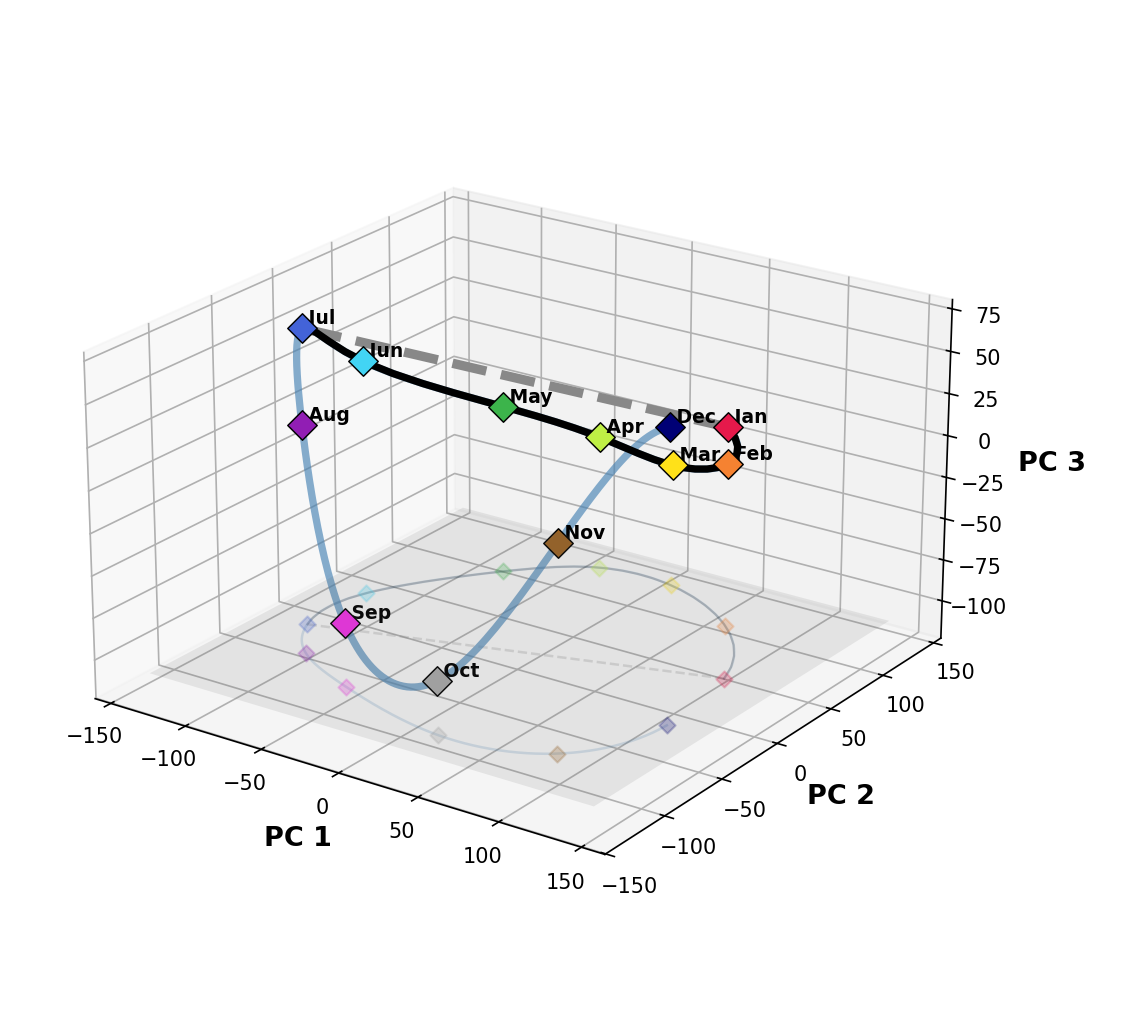
\includegraphics[width=0.255\textwidth,trim=0 0 0 55pt,clip]{figures/months_activation.png}\\
    
\includegraphics[width=0.34\textwidth]{figures/weekdays_probs.png} &
    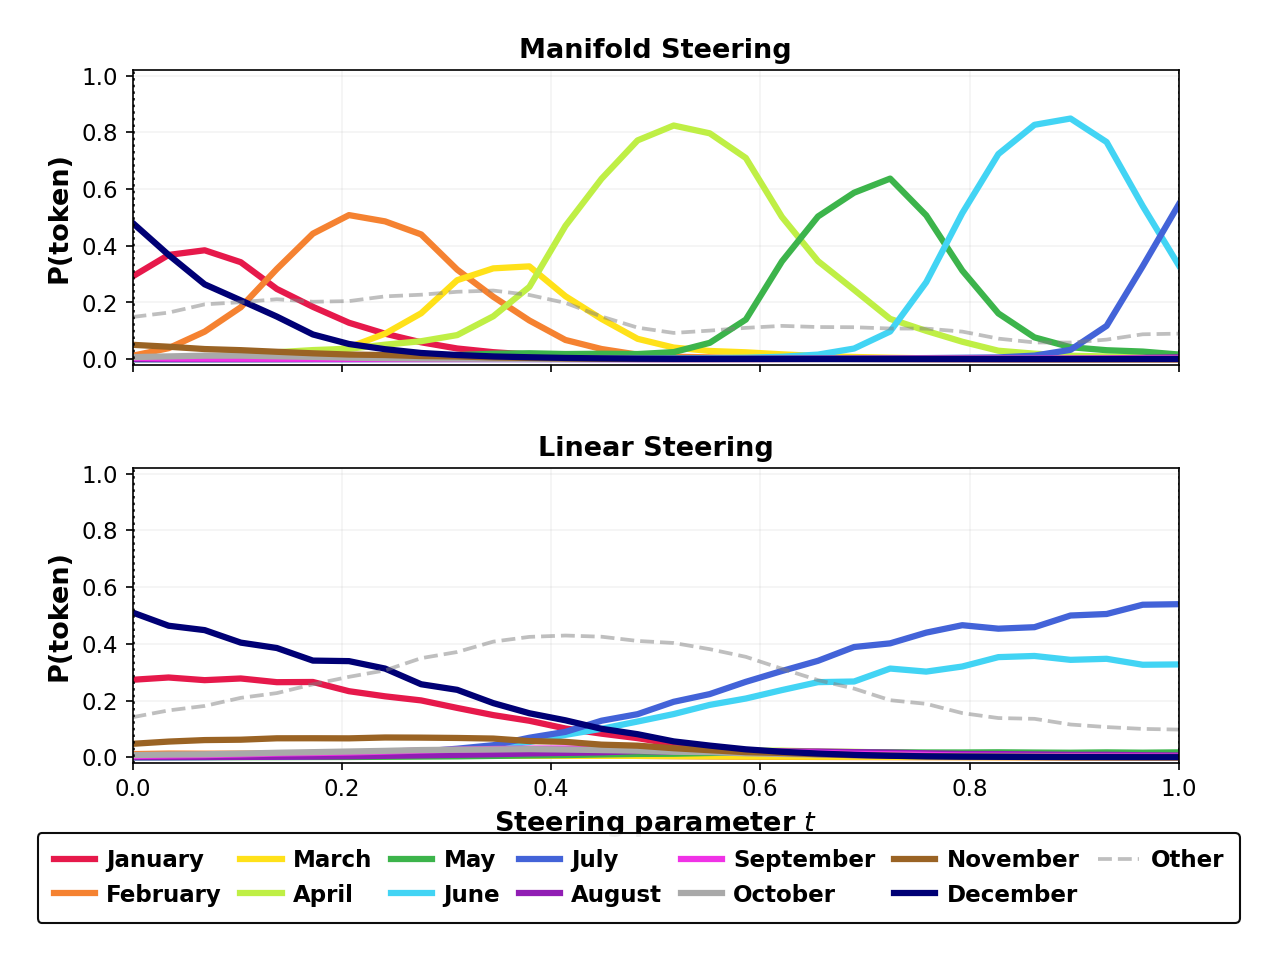
\includegraphics[width=0.34\textwidth]{figures/months_probs.png}\\
  \end{tabular}
  \caption{Gemma-2-2B layer 24, steering Tue$\to$Fri (weekdays) and
  Jan$\to$Jul (months). Rows 1--2: fitted behavior manifolds $\mathcal{M}_y$
  (Hellinger--PCA) and activation manifolds $\mathcal{M}_h$ (activation--PCA)
  with the linear path (dashed) and manifold path (black). Row 3:
  concept-token probabilities along each path.}
  \label{fig:main}
\end{figure}

\section{The experiment, step by step}

\textbf{Setup.} All experiments use instruction-tuned \textbf{Gemma-2-2B}
($d=2304$), patching layer 24 of 26. Two cyclic concept domains:
\emph{weekdays} (7 classes) and \emph{months} (12 classes), probed with
arithmetic prompts --- ``\texttt{Q: What day is two days after Monday? A:}''
(answer: \emph{Wednesday}), 6 prompts per concept
(\texttt{scripts/run\_weekdays.py}, \texttt{run\_months.py}). For each prompt
we record the last-token hidden state $h^{(24)}$ and the output distribution
over concept tokens, then average per concept:
$\hat h_c = \tfrac{1}{N_c}\sum_{i\in S_c} h^{(L)}_i$ and
$\hat p_c = \tfrac{1}{N_c}\sum_{i\in S_c} p_i$.

\textbf{Manifolds.} A ``manifold'' here is simply a smooth curve through the
concept centroids. The 7 weekday centroids $\hat h_{c_k}\in\mathbb{R}^{2304}$
span at most a 6-dimensional subspace, so PCA to $r{=}6$ ($r{=}11$ for 12
months) is lossless --- it just re-expresses each centroid in coordinates
$z_k\in\mathbb{R}^r$ adapted to the data. We then fit a cubic spline
$\gamma:\mathbb{R}\to\mathbb{R}^r$ through the points \emph{in concept
order}, with the concept index as curve parameter: $\gamma(k)=z_k$ exactly at
each knot, and between knots
$\gamma(t)=a_k+b_k(t{-}k)+c_k(t{-}k)^2+d_k(t{-}k)^3$, coefficients solved
jointly so the curve is $C^2$-smooth. This gives the activation manifold
$\mathcal{M}_h$: a single scalar coordinate (``where between Monday and
Sunday'') decodes to a full hidden state via
$\mathrm{PCA}^{-1}(\gamma(t))$. The behavior manifold $\mathcal{M}_y$ is
built identically from the probability centroids, except each $\hat p_{c_k}$
is first mapped to $\sqrt{\hat p_{c_k}}$ (Hellinger space), where Euclidean
tools --- PCA, splines, distances --- respect the geometry of the probability
simplex.

\textbf{Steering.} For $\alpha\in[0,1]$ between spline indices $i_s,i_e$:
$\pi_{\mathrm{mfd}}(\alpha)=\mathrm{PCA}^{-1}\!\big(\gamma(i_s+\alpha\,\Delta
i)\big)$. At each of 30 steps, a forward hook replaces the layer-24 hidden
state at the last token with $\pi(\alpha_t)$ and the output probability of
every concept token is recorded (\texttt{scripts/run\_steering\_probs.py}).
Everything is deterministic; all figures regenerate from committed
checkpoints without a GPU (see the repo README).

\section{Replication of the main figure}

Figure~\ref{fig:main} replicates the paper's main result. In both domains the
concept centroids trace closed, ordered loops in activation space and in
behavior space --- the cyclic structure of weeks and months is visibly
encoded. The manifold path stays on the fitted curve and, in the probability
trajectories (row 3), produces \emph{smooth, ordered} transitions: steering
from Tuesday to Friday passes probability mass through Wednesday and Thursday
in sequence. Linear steering instead leaves the manifold and
\emph{teleports}: intermediate concepts never rise in order, and off-concept
mass appears mid-path. One practical lesson: patch deep enough --- at layer
12, keys/values from the original prompt override the patch over the 14
remaining blocks and both methods flatline; layer 24 (92\% depth) is clean.

\section{Extension: torus steering (day $\times$ hour)}

Do LLMs encode \emph{two-dimensional} concept structure? A weekday lives on
one circle; a (day, hour) pair lives on a \emph{product} of two circles ---
a torus. We collect layer-24 activations for all 168 prompts ``\texttt{It is
HH:00 on \{Day\}}'' (7 days $\times$ 24 hours) and assign each prompt two
angles, $\theta_{\mathrm{day}}=2\pi k/7$ and $\theta_{\mathrm{hour}}=2\pi
h/24$. Each circle's 2D subspace
$V_{\mathrm{day}},V_{\mathrm{hour}}\in\mathbb{R}^{2\times d}$ is recovered by
regressing centered activations onto the standardized labels
$[\sin\theta,\cos\theta]$ --- each label component yields one direction
$d\propto\sum_i (h_i-\bar h)\,\ell_i$ --- followed by QR-orthogonalization of
the two directions (\texttt{scripts/run\_hierarchical\_steering.py}). The two
recovered planes are nearly orthogonal to each other (max
$|\cos|\approx0.18$), so day and hour occupy largely independent planes of
the residual stream. Projecting each activation onto both planes gives two recovered angles,
rendered on a torus --- day on the major circle, hour on the minor
(Fig.~\ref{fig:torus}, left). The 7 day-arcs are cleanly ordered; the hour
circle does not fully close, so hour is only partially circular here.

\begin{figure}[b!]
  \centering
  \begin{minipage}[c]{0.44\textwidth}
    \centering
    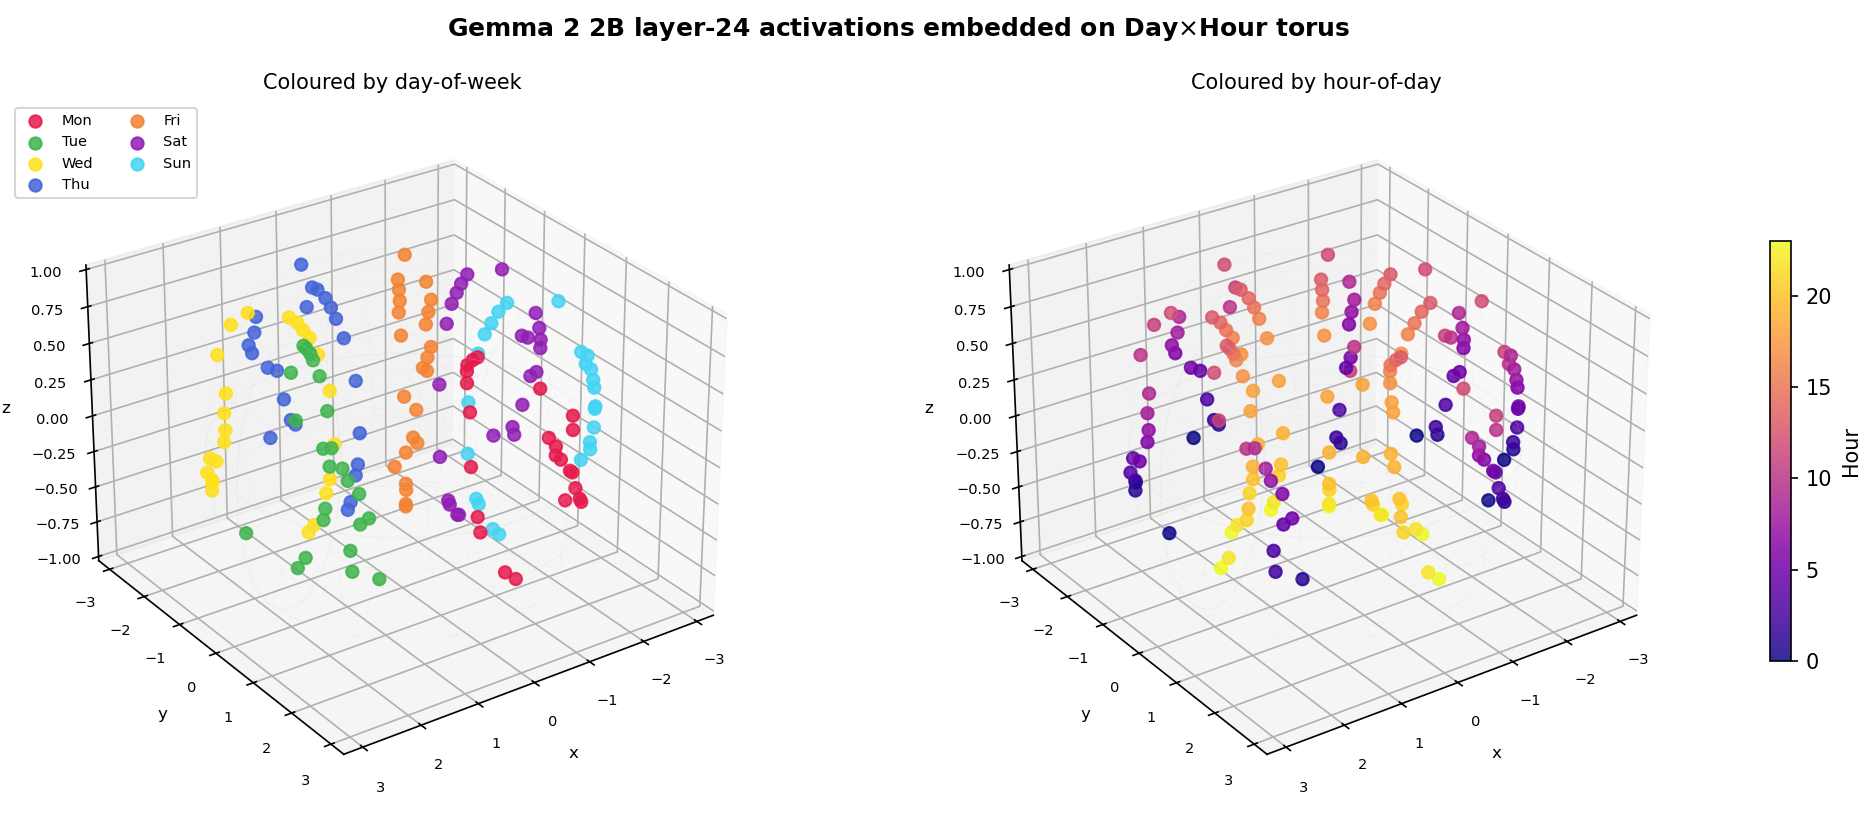
\includegraphics[width=\linewidth,trim=0 0 0 48pt,clip]{figures/torus_repr.png}
  \end{minipage}\hfill
  \begin{minipage}[c]{0.50\textwidth}
    \centering
    
\includegraphics[width=\linewidth,trim=0 0 0 44pt,clip]{figures/subspace_2d_grid.png}
  \end{minipage}
  \caption{\textbf{Left:} layer-24 activations on the day$\times$hour torus,
  colored by day (7 ordered arcs) and by hour. \textbf{Right:}
  day$\times$hour probability grids across 6 steering steps, (Tue,\,09:00)
  $\to$ (Fri,\,15:00); top row torus (product-coordinate) steering, bottom
  row linear steering.}
  \label{fig:torus}
\end{figure}

Steering in \emph{product coordinates} respects this factorization: starting
from the source activation $h_{\mathrm{base}}$ (Tue, 09:00), each step moves
the day and hour coordinates \emph{independently within their own planes},
$h(\alpha) = h_{\mathrm{base}} +
\Delta_{\mathrm{day}}(\alpha)\,V_{\mathrm{day}} +
\Delta_{\mathrm{hour}}(\alpha)\,V_{\mathrm{hour}}$, where
$\Delta_c(\alpha)$ interpolates the source$\to$target offset within each
plane --- the 2D analogue of walking along the manifold. Each patched activation is decoded into a day$\times$hour probability grid:
day from token probabilities, hour by nearest centroid in the
$V_{\mathrm{hour}}$ plane (two-digit hours are multi-token for Gemma, so
subspace readout is more faithful). Steering (Tue,\,09:00) $\to$
(Fri,\,15:00) over six steps (Fig.~\ref{fig:torus}, right), the bright cell
walks diagonally --- both coordinates move smoothly --- while linear steering
moves the day correctly but teleports the hour, jumping to 15:00 only at the
final step: the same off-manifold failure mode, now visible per coordinate.

\textbf{Takeaway.} Representation geometry is not decoration: moving along
it produces natural behavior, and ignoring it breaks transitions exactly as
the manifold picture predicts. Code, checkpoints, and full reproduction
instructions: \url{\repourl}.

\section{References}

{\small
[1] D.~Wurgaft, C.~Rager, M.~Kowal, V.~Shyam, S.~Feucht, U.~Bhalla,
T.~Haklay, E.~Bigelow, R.~Sarfati, T.~McGrath, O.~Lewis, J.~Merullo,
N.~D.~Goodman, T.~Fel, A.~Geiger, and E.~S.~Lubana. Manifold steering
reveals the shared geometry of neural network representation and behavior.
\emph{arXiv preprint arXiv:2605.05115}, 2026.

[2] S.~Amari and H.~Nagaoka. \emph{Methods of Information Geometry}.
American Mathematical Society, 2000.}

\end{document}
